\documentclass[12pt, a4paper, oneside]{ctexart}
\usepackage{amsmath, amsthm, amssymb, bm, color, framed, graphicx, hyperref, mathrsfs}

\title{\textbf{9月17日作业}}
\author{韩岳成 524531910029}
\date{\today}
\linespread{1.5}
\definecolor{shadecolor}{RGB}{241, 241, 255}
\newcounter{problemname}
\newenvironment{problem}{\begin{shaded}\stepcounter{problemname}\par\noindent\textbf{题目\arabic{problemname}. }}{\end{shaded}\par}
\newenvironment{solution}{\par\noindent\textbf{解答. }}{\par}
\newenvironment{note}{\par\noindent\textbf{题目\arabic{problemname}的注记. }}{\par}

\begin{document}

\maketitle

\begin{problem}
设 A,B,C 为三个事件,试用事件的关系和运算表示下列事件:

(1) 只有 A 发生;

(2) A 与 B 都发生而 C 不发生;

(3) A,B,C 都不发生;

(4) A,B,C 不都发生;

(5) A.B,C 中至少有一个发生.
\end{problem}

\begin{solution}
(1) $A\,\overline{B}\,\overline{C}$

(2) $A\,B\,\overline{C}$

(3) $\overline{A}\,\overline{B}\,\overline{C}=\overline{A\cup B\cup C}$

(4) $\overline{ABC}$

(5) $A\cup B\cup C$
\end{solution}

\begin{problem}
甲、乙二人参加知识竞赛,共有10道不同的题目其中有6道选择题,4道判断题.甲、乙二人依次各抽1题.

(1) 求甲抽到选择题,乙抽到判断题的概率;

(2) 求甲、乙二人中至少有一人抽到选择题的概率.
\end{problem}

\begin{solution}
设事件A为甲抽到选择题,事件B为乙抽到判断题,则

(1) $P(A)=\frac{6}{10}=\frac{3}{5}$, $P(B|A)=\frac{4}{9}$,

$P(AB)=P(A)P(B|A)=\frac{4}{15}$.

(2) $P(\overline{A})=1-P(A)=\frac{2}{5}, P(B|\overline{A})=\frac{3}{9}=\frac{1}{3}$

$P(\overline{A}B)=P(\overline{A})P(B|\overline{A})=\frac{2}{15}$

$P(A\cup \overline{B})=1-P(\overline{A}B) = \frac{13}{15}$
\end{solution}

\begin{problem}
假设某博彩中心发行了n张奖券,其中 m$(m\le n)$张有奖.某人一次性买了k($k\le n$) 张奖券,这k张中没有一张有奖的概率是多少?这k张中多于两张有奖的概率是多少?
\end{problem}

\begin{solution}
设没有一张有奖为事件A,有一张有奖为事件B,有两张有奖为事件C。

当$k\le n-m$时,$P(A)=\frac{C_{n-m}^k}{C_n^k}$,

当$k > n-m$时, $P(A)=0$.

当$k \le n-m+1$且$m \ge 1$时, $P(B)=\frac{C_{n-m}^{k-1}C_m^1}{C_n^k}$,

当$k > n-m+1$时,$P(B)=0$;

当$k \le n-m+2$且$m \ge 2$时,$P(C)=\frac{C_{n-m}^{k-2}C_m^2}{C_n^k}$,

当$k > n-m+2$时,$P(C)=0$

因此$P(\overline{A}\,\overline{B}\,\overline{C}) = 1-P(A)-P(B)-P(C) \\= \left\{\begin{matrix}1-\frac{C_{n-m}^k+C_{n-m}^{k-1}C_m^1+C_{n-m}^{k-2}C_m^2}{C_n^k},&k \le n-m+3,m\ge3,\\1,&k > n-m+3,m\ge3,\\0,&m<3.\end{matrix}\right.$
\end{solution}

\begin{problem}
有放回地从数字 1,2,...,n 中随机抽取 k 个数($k\le n$),求下列事件的概率:

(1) A 表示事件“k个数字全不相同”;

(2) B 表示事件“数字‘5’恰好出现 r 次”($r\le k$);

(3) C 表示事件“至少出现r个数字‘5’”($r \le k$).
\end{problem}

\begin{solution}
(1) $P(A)= \frac{A_n^k}{n^k}$;

(2) $P(B)=\frac{C_k^r (n-1)^{k-r}}{n^k}$;

(3) $P(C)=\frac{\sum_{i=r}^k C_k^i (n-1)^{k-i}}{n^k}$.
\end{solution}

\begin{problem}
甲、乙二人约定上午 9:00 至 9:20 之间到某地铁站乘地铁,这段时间内有4 班车,开车时间分别为 9:05, 9: l0, 9: 15, 9: 20.他们约定 (l) 见车就乘 ;(2) 最多等一班车.假设甲、乙到达地铁站的时刻互不影响,且每人在这段时间内任何时刻到达车站是等可能的、求甲、乙同乘一班车的概率.
\end{problem}
\begin{solution}
设甲、乙同乘一班车为事件A,甲、乙到达地铁站的时刻距9:00分别为x,y,

$\Omega=\{(x,y)|0\le x,y\le 20\}$.

(1) 事件A对应的区域如下图所示:
\begin{figure}[h]
    \centering
    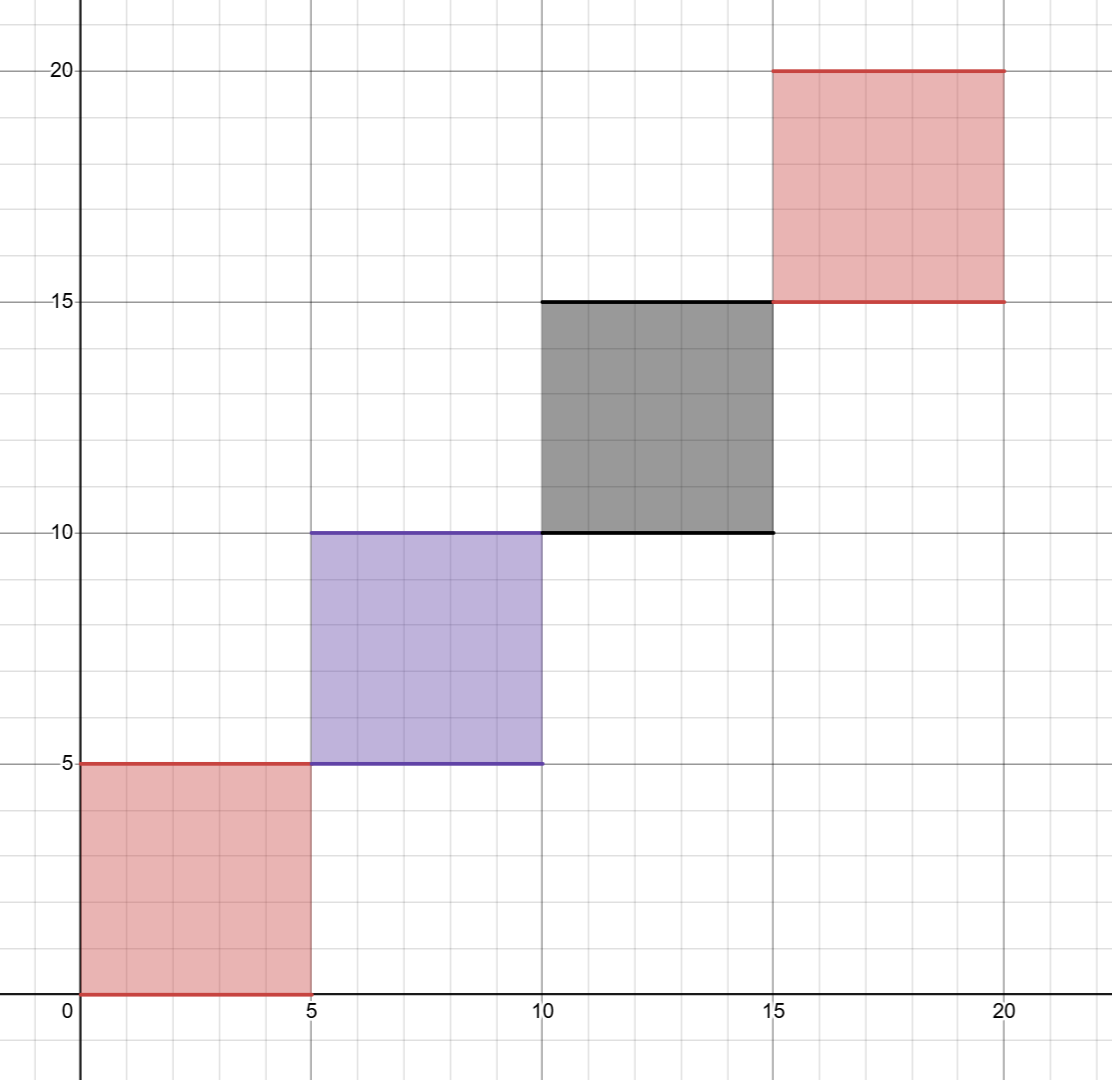
\includegraphics[width=0.5\linewidth]{image1.png}
\end{figure}

因此$P(A)=\frac{4}{16}=\frac{1}{4}$.

(2) 事件A对应的区域如下图所示:
\begin{center}
    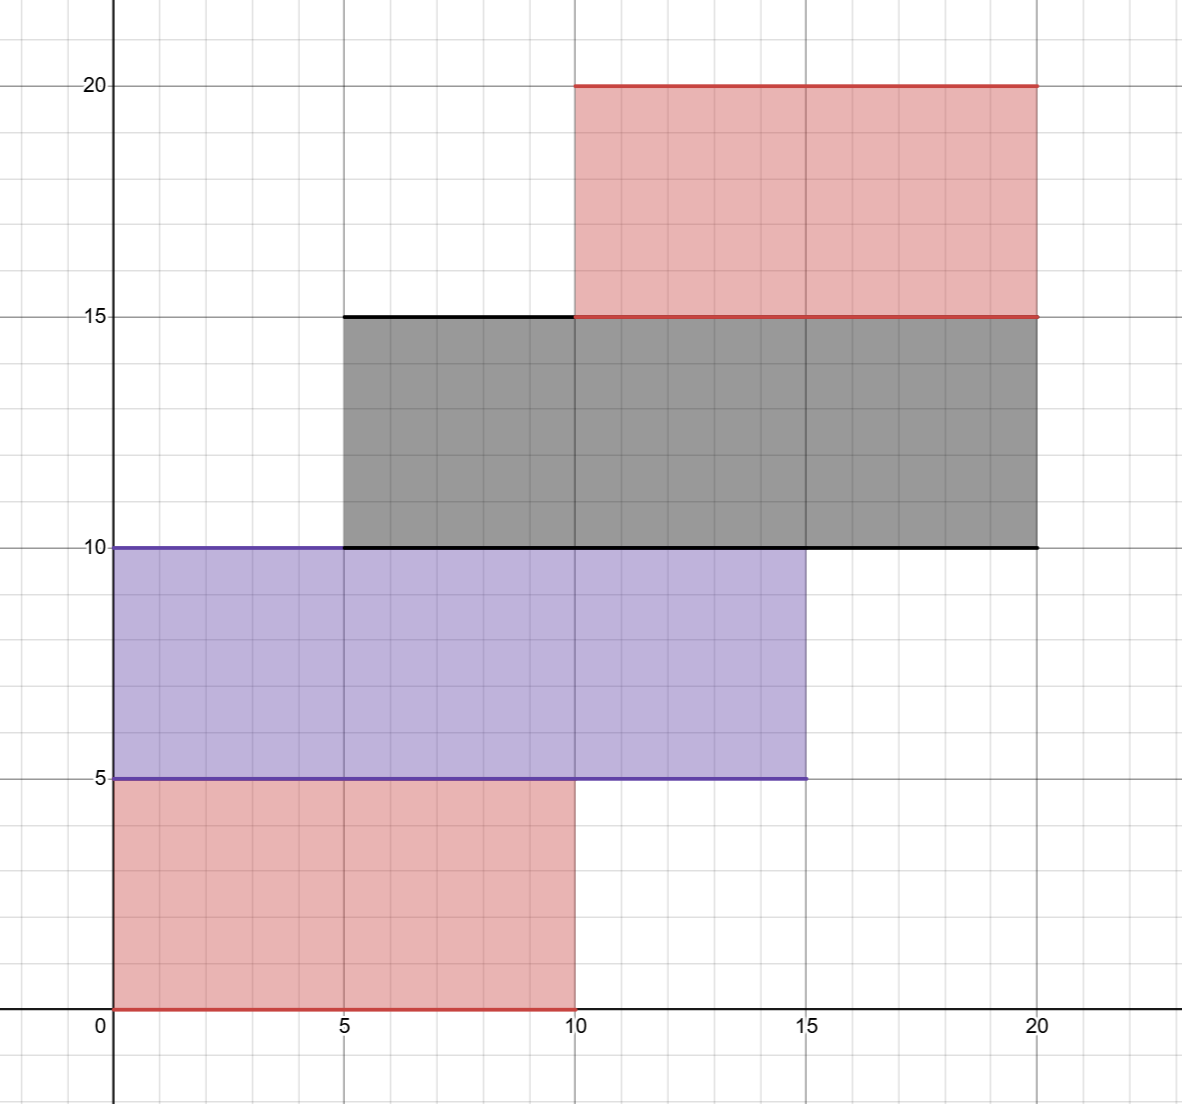
\includegraphics[width=0.5\linewidth]{image2.png}
\end{center}

因此 $P(A)=\frac{10}{16}=\frac{5}{8}$.

\end{solution}

\begin{problem}
考虑一元二次方程$x^2+Bx+C=0$,其中B,C分别是将一枚骰子接连投掷两次先后出现的点数。求该方程有实根的概率和该方程有重根的概率。
\end{problem}

\begin{solution}
设该方程有实根为事件A,该方程有重根为事件B.

样本空间$\Omega=\{(1,1),(1,2),...,(1,6),(2,1),(2,2),...,(2,6),...,(6,6)\}$.

当$B^2-4C\ge0$时,该方程有实根,因此$A=\{(2,1),(3,1),(3,2),(4,1),(4,2),\\(4,3),(4,4),(5,1),(5,2),(5,3),(5,4),(5,5),(5,6),(6,1),(6,2),(6,3),(6,4),(6,5),\\(6,6)\}$,$P(A)=\frac{19}{36}$.

当$B^2-4C=0$时,该方程有重根,因此$B=\{(2,1),(4,4)\}$,$P(B)=\frac{2}{36}=\frac1{18}$.
\end{solution}
\end{document}